After establishing a theoretical foundation on both multigrid methods and evolutionary program synthesis, we can now focus on developing a formal language for expressing arbitrarily-structured multigrid solvers in a generalized way.
As we have seen in Section~\ref{sec:multigrid-cycles}, according to the classical formulation of multigrid, each of these methods belongs to a particular class of cycles.
Each cycle possesses a distinct computational structure that stems from the number of recursive descents performed on each level of the method, as determined by the parameter $\gamma$ in Algorithm~\ref{alg:multigrid-cycle}.
For instance, a V-cycle is characterized by exactly one recursive descent per level.
Furthermore, each classical multigrid cycle employs a fixed number of smoothing steps per discretization level, which is determined by the parameters $\nu_1$ and $\nu_2$.
While the representation of a multigrid method as a recursive cycle yields a formally simple and easily parameterizable algorithmic formulation, it also enforces unnecessary restrictions on its structure.
Consider, for instance, the multigrid method shown in Figure~\ref{fig:non-traditional-multigrid-cycle}.
\begin{figure}
		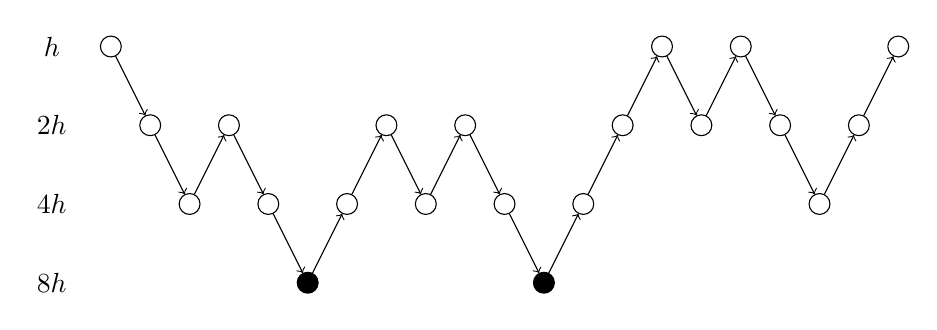
\begin{tikzpicture}
            \node   (h) at (-0.75, 4){$h$};
			\node   (2h) at (-0.75, 3){$2h$};
			\node   (4h) at (-0.75, 2){$4h$};
			\node   (8h) at (-0.75, 1){$8h$};
			\node	(a) at (0,4) [draw, circle,scale=0.8] {};
			\node	(b) at (0.5,3) [draw, circle,scale=0.8] {};
			\node	(c) at (1,2) [draw, circle,scale=0.8] {};
			\node	(d) at (1.5,3) [draw, circle, scale=0.8] {};
			\node	(e) at (2,2) [draw, circle, scale=0.8] {};
			\node	(f) at (2.5,1) [draw, circle,scale=0.8,fill=black] {};
			\node	(g) at (3,2) [draw, circle,scale=0.8] {};
			\node	(h) at (3.5,3) [draw, circle,scale=0.8] {};
			\node	(i) at (4,2) [draw, circle,scale=0.8] {};
			\node	(j) at (4.5,3) [draw, circle,scale=0.8] {};
			\node	(k) at (5,2) [draw, circle,scale=0.8] {};
			\node	(l) at (5.5,1) [draw, circle,scale=0.8,fill=black] {};
			\node	(m) at (6,2) [draw, circle,scale=0.8] {};
			\node	(n) at (6.5,3) [draw, circle,scale=0.8] {};
			\node	(o) at (7,4) [draw, circle,scale=0.8] {};
			\node	(p) at (7.5,3) [draw, circle,scale=0.8] {};
			\node	(q) at (8,4) [draw, circle,scale=0.8] {};
			\node	(r) at (8.5,3) [draw, circle,scale=0.8] {};
			\node	(s) at (9,2) [draw, circle,scale=0.8] {};
			\node	(t) at (9.5,3) [draw, circle,scale=0.8] {};
			\node	(u) at (10,4) [draw, circle,scale=0.8] {};
			\draw 
			(a) edge[->] (b) 
			(b) edge[->] (c)
			(c) edge[->] (d)
			(d) edge[->] (e)   
			(e) edge[->] (f)
			(f) edge[->] (g)
			(g) edge[->] (h)
			(h) edge[->] (i)
			(i) edge[->] (j)
			(j) edge[->] (k)
			(k) edge[->] (l)
			(l) edge[->] (m)
			(m) edge[->] (n)
			(n) edge[->] (o)
			(o) edge[->] (p)
			(p) edge[->] (q)
			(q) edge[->] (r)
			(r) edge[->] (s)
			(s) edge[->] (t)
			(t) edge[->] (u)
			;
		\end{tikzpicture}
	\caption{Example for a non-classical multigrid method.}
	\label{fig:non-traditional-multigrid-cycle}
\end{figure}
While this method reaches the coarsest level twice and, hence, at first sight, looks similar to a W-cycle, it employs a unique pattern of computations that is completely different from any known multigrid cycle.
As a consequence, this method can not be represented within the classical framework of multigrid cycles, as formulated in Algorithm~\ref{alg:multigrid-cycle}.
To overcome the limitations of this formulation by constructing multigrid methods with a unique sequence of computations on each discretization level, a new formal language is needed.
The first step toward the development of such a language is to find a way to represent the state within each step of a multigrid method.
Based on this representation, we can then define transition rules between the individual states, which will allow us to design multigrid methods of novel structure.
\section{Multigrid States}
\label{sec:multigrid-states}
In order to derive a representation of the state of a multigrid method, we need to reconsider our original formulation of a multigrid cycle in Algorithm~\ref{alg:multigrid-cycle}.
For the sake of simplicity, in the following, symbols that correspond to vectors are written in regular font.
In case the mathematical interpretation of a certain lowercase symbol is ambiguous, its meaning will be explicitly stated. 
With the exception of the coarsest level, where the only allowed operation is the application of the coarse-grid solver, we can identify three elementary multigrid operations that can be performed within a cycle.
\begin{definition}[Elementary Multigrid Operations]
\label{def:elementary-multigrid-operations}
On each level except for the lowest, the following three operations can be performed within a multigrid cycle.
\begin{itemize}
	\item \textbf{Smoothing}: Reduce the oscillatory error components of the approximate solution $\tilde{x}_h$ on the current level. 
	\begin{equation}
		\tilde{x}_h = \tilde{x}_h + \omega M_h^{-1} \left( b_h - A_h \tilde{x}_h \right) \; \text{where} \; A_h = M_h + N_h
	\end{equation}
	\item \textbf{Coarsening}: A coarse problem is obtained by restricting the residual.
	\begin{equation}
    \begin{split}
     	\tilde{x}_{2h} & = 0 \\
		b_{2h} & = I_h^{2h} (b_h - A_h \tilde{x}_h)
    \end{split}
	\end{equation}
	\item \textbf{Coarse-Grid Correction}: Prolongate a correction $\tilde{x}_{2h}$ obtained on a coarser grid to reduce the low-frequency error components of the approximate solution $\tilde{x}_h$.
	\begin{equation}
		\tilde{x}_h = \tilde{x}_h + I_{2h}^h \tilde{x}_{2h}
	\end{equation}
\end{itemize}
\end{definition}
Except for the operators $A_h$, $I_h^{2h}$ and $I_{2h}^h$ the result of each of these operations exclusively depends on the current value of the approximate solution on subsequent levels, i.e., $\tilde{x}_{h}$ and $\tilde{x}_{2h}$, and the right-hand side $b_h$.
However, in contrast to the coarse-grid correction step, which makes use of the current approximate solution on the coarse grid, both smoothing as well as coarsening requires us first to compute the residual $r_h = b_h - A_h \tilde{x}_h$, which can be considered as an intermediate step.
While this differentiation is not strictly necessary, it leads to simpler expressions since both operations can then be split into two steps.
Furthermore, as in practice, the error can usually not be computed directly, the residual is often the only available metric to investigate whether a multigrid iteration has achieved a certain amount of error reduction and, hence, has to be computed repeatedly.
%The residual is then either restricted and assigned to the right-hand side $b_{2h}$ or employed to reduce the oscillatory error components of the approximate solution by computing a coarse-grid correction term of the form $\omega A_h^{-1} r_h$.
To derive a general representation for the state of a multigrid method based on our previous observations, we next consider the sequence of operations shown in Algorithm~\ref{alg:example-three-grid-method}, which corresponds to a three-grid V-cycle that performs one step of underrelaxed Jacobi smoothing on the second finest level.
\begin{algorithm}
	\begin{algorithmic}[1]
		\State $\tilde{x}_{h} = x_{h}^{0}$
		\State $r_{h} = b_{h} - A_h \tilde{x}_{h} $
		\State $ \tilde{x}_{2h} = 0$
		\State $ b_{2h} = I_{h}^{2h} r_{h}$
		\State $ r_{2h} = b_{2h} - A_{2h} \tilde{x}_{2h}$
		\State $ \tilde{x}_{2h} = \tilde{x}_{2h} + I_{4h}^{2h} A_{4h}^{-1} I_{2h}^{4h} r_{2h}$
		\State $ r_{2h} = b_{2h} - A_{2h} \tilde{x}_{2h}$
		\State $ \tilde{x}_{2h} = \tilde{x}_{2h} + 0.6 \cdot D_{2h}^{-1} r_{2h}$
		\State $\tilde{x}_{h} = \tilde{x}_{h}  + I_{2h}^h \tilde{x}_{2h}$
	\end{algorithmic}
\caption{Example for a three-grid V-cycle}
\label{alg:example-three-grid-method}
\end{algorithm}
In each step of this sequence, either the approximate solution, right-hand side, or residual is updated on a particular level.
While in practice, each of these variables corresponds to a data structure comprising numerical values, our goal is to represent the algorithmic structure of a multigrid method in the form of symbolic expressions.
In this case, the value of each variable is determined by the expression that computes its value.
Updating a variable, therefore, corresponds to assigning a new expression to the corresponding symbol.
For this purpose, we consider the tuple
\begin{equation*}
	Z_h = (\tilde{x}_h, b_h, r_h)
\end{equation*} 
on each level with step size $h$, which then refers to the expression of each of the corresponding three variables.
Starting from the first line, we can progressively update the contents of this tuple with the expression given in each line, whereby each occurrence of one of the three symbols is replaced by the expression currently contained in the respective entry of the tuple.
Figure~\ref{fig:example-tree-grid-method-states} shows the content of the state tuple for each line of Algorithm~\ref{alg:example-three-grid-method}.
\begin{figure}
	\begin{equation*}
		\begin{array}{l l}
			\hline
			\bm{Z_h} & \bm{(\tilde{x}_h, \, b_h, \, r_h)}  \\
			1: &  x_{h}^0, \, b_h, \, \lambda \\
			2: &  x_{h}^0, \, b_h, \, b_{h} - A_h x_{h}^0 \\ \hline
			\bm{Z_{2h}} &  \bm{(\tilde{x}_{2h}, \, b_{2h}, \, r_{2h})} \\
			3: &  0, \, \lambda, \, \lambda \\
			4: &  0, \, I_{h}^{2h}\underbrace{(b_{h} - A_h x_{h}^0)}_{r_{h}}, \, \lambda \\
			5: &  0, \, I_{h}^{2h}(b_{h} - A_h x_{h}^0), \,\underbrace{I_{h}^{2h}(b_{h} - A_h x_{h}^0)}_{b_{2h}} - A_{2h} 0 \\
			6: & 0 + I_{4h}^{2h} A_{4h}^{-1} I_{2h}^{4h} (\underbrace{I_{h}^{2h}(b_{h} - A_h x_{h}^0) - A_{2h} 0}_{r_{2h}}), \, I_{h}^{2h}(b_{h} - A_h x_{h}^0), \, \lambda\\
			7: & 0 + I_{4h}^{2h} A_{4h}^{-1} I_{2h}^{4h} (I_{h}^{2h}(b_{h} - A_h x_{h}^0) - A_{2h} 0), \, I_{h}^{2h}(b_{h} - A_h x_{h}^0), \\ 
			&  \underbrace{I_{h}^{2h}(b_{h} - A_h x_{h}^0)}_{b_{2h}} - A_{2h} (\underbrace{0 + I_{4h}^{2h} A_{4h}^{-1} I_{2h}^{4h} (I_{h}^{2h}(b_{h} - A_h x_{h}^0) - A_{2h} 0)}_{\tilde{x}_{2h}}) \\
			8: &   (\underbrace{0 + I_{4h}^{2h} A_{4h}^{-1} I_{2h}^{4h} (I_{h}^{2h}(b_{h} - A_h x_{h}^0) - A_{2h} 0)}_{\tilde{x}_{2h}}) + 0.6 \cdot D_{2h}^{-1} \cdot \\ 
			& (\underbrace{I_{h}^{2h}(b_{h} - A_h x_{h}^0) - A_{2h} (0 + I_{4h}^{2h} A_{4h}^{-1} I_{2h}^{4h} (I_{h}^{2h}(b_{h} - A_h x_{h}^0) - A_{2h} 0))}_{r_{2h}}), \\ 
			& I_{h}^{2h}(b_{h} - A_h x_{h}^0), \, \lambda \\ \hline 
			\bm{Z_h} & \bm{(\tilde{x}_h, \, b_h, \, r_h)}  \\
			9: & x_{h}^0 + I_{2h}^h ((0 + I_{4h}^{2h} A_{4h}^{-1} I_{2h}^{4h} (I_{h}^{2h}(b_{h} - A_h x_{h}^0) - A_{2h} 0)) + 0.6 \cdot D_{2h}^{-1} \cdot \\ 
			& (I_{h}^{2h}(b_{h} - A_h x_{h}^0) - A_{2h} (0 + I_{4h}^{2h} A_{4h}^{-1} I_{2h}^{4h} (I_{h}^{2h}(b_{h} - A_h x_{h}^0) - A_{2h} 0)))), \\ 
			&  b_h, \, \lambda \\
			\hline
		\end{array}
	\end{equation*}
	\caption{State tuple in each step of Algorithm~\ref{alg:example-three-grid-method}.}
	\label{fig:example-tree-grid-method-states}
\end{figure}
As introduced in Section~\ref{sec:formal-languages}, the empty symbol $\lambda$ denotes that a certain component of the tuple is unspecified.
After the last step of the sequence (Line~9), the first component $\tilde{x}_h$ of the tuple combines all computational steps of the method in a single expression.

While Figure~\ref{fig:example-tree-grid-method-states} illustrates that the ternary tuple $Z_h$ contains all relevant information of a multigrid method's current state on a certain level, we have not yet discussed how we can transition between the states of two subsequent levels.
First, we consider the case of transitioning from a level with step size $h$ to the next coarser grid with step size $2h$, which is shown in Line~3~and~4 of Figure~\ref{fig:example-tree-grid-method-states}.
Here, the tuple
\begin{equation*}
	Z_{2h} = (0, \, I_{h}^{2h}(b_{h} - A_h x_{h}^0), \, \lambda)
\end{equation*} 
corresponds to the coarse-grid error equation 
\begin{equation*}
	A_{2h} x_{2h} = I_{h}^{2h}(b_{h} - A_h x_{h}^0),
\end{equation*}
whose solution is to be approximated, starting with an initial guess of zero.
Therefore, all necessary information for the creation of this state is obtained from the next higher level in the form of the restricted residual 
\begin{equation*}
    I_h^{2h} r_h = I_h^{2h} (b_{h} - A_h x_{h}^0).
\end{equation*}
On the other hand, consider the transition from a coarse grid back to the next finer grid in the form of the coarse-grid correction in Line~9.
In this case, we require both the approximate solution $\tilde{x}_{2h}$, computed on the coarse grid, as well as the previous values of the first two entries of the fine-grid state tuple, i.e., $\tilde{x}_h$ and $b_h$.
While for coarsening, we can neglect all previous states on the coarser grid, as their information is explicitly contained in the residual, for a coarse-grid correction, the previous state on the fine grid needs to be restored.
Note that for a multigrid method that operates on a hierarchy of discretizations of even larger depth than the example shown in Algorithm~\ref{alg:example-three-grid-method}, this process must be carried out recursively for each bottom-up transition.
To resolve this issue, we need to extend our original formulation of a multigrid state with a fourth component that has the purpose of preserving the current state on the next-higher level.
While at the topmost level, this component is always empty, whenever coarsening is performed, the state of the current level is included.
For instance, in Line~4 of Figure~\ref{fig:example-tree-grid-method-states} we have to extend the given ternary tuple 
\begin{equation*}
Z_{2h} = (0, \, I_{h}^{2h}(b_{h} - A_h x_{h}^0), \, \lambda)
\end{equation*}
by including the state 
\begin{equation*}
Z_h = (x_{h}^0, \, b_h, \, \lambda, \, \lambda) 
\end{equation*} 
as an additional fourth entry. 
As a consequence, all required information for restoring the previous fine-grid state values is included in the quaternary tuple 
\begin{equation*}
	Z_{2h} = (0, \, I_{h}^{2h}(b_{h} - A_h x_{h}^0), \, \lambda, \, Z_h).
\end{equation*}
Note that since $Z_h$ represents the current state on the finest grid, its fourth component is empty, while otherwise, it would refer to the previous state of the next higher level in the discretization hierarchy.
To assess the feasibility of this approach, we have to check whether all components required to construct the coarse-grid correction expression, as in Line~9 of Figure~\ref{fig:example-tree-grid-method-states}, are available within the current state.
Since in addition to $\tilde{x}_{2h}$, both the approximate solution $\tilde{x}_h$ and right-hand side $b_h$ are now contained in the fourth component of the coarse-grid state tuple, this expression can be assembled in a straightforward manner.
At this point, note that a coarse-grid correction on the lowest level represents a special case. 
Since the only allowed operation on this level is the application of the coarse-grid solver, which is denoted by multiplication with the inverse of the system matrix, it is represented as a single operation given by the expression 
\begin{equation*}
	\tilde{x}_{2h} = \tilde{x}_{2h} + I_{4h}^{2h} A_{4h}^{-1} I_{2h}^{4h} r_{2h}.
\end{equation*}
After resolving the issue of restoring previous states during a coarse-grid correction, we can thus provide a complete formal definition of the state of a multigrid method.
\begin{definition}[Multigrid State]
\label{def:multigrid-state}
The state of a multigrid method for solving the equation $A_{h} x_{h} = b_{h}$ on a grid with step size $h$ is given by the quaternary tuple
\begin{equation}
	Z_{h} = \left( \tilde{x}_{h}, b_{h}, c_{h}, Z_{h/2}\right), 
\end{equation}
where
\begin{itemize}
	\item $\tilde{x}_{h}$ is a mathematical expression for computing an approximate solution of the above equation,
	\item $b_{h}$ is an expression for computing the right-hand side of the above equation,
	\item $c_{h}$ is a correction term for improving the accuracy of the approximate solution,
	\item $Z_{h/2}$ is either the current state on the next finer grid with a step size $h/2$ or the empty symbol $\lambda$ in case $h$ represents the topmost level in the given hierarchy of discretizations.
\end{itemize}
\end{definition}
Note that in Definition~\ref{def:multigrid-state}, the third component $c_{h}$ of a multigrid state no longer has to refer to the residual but now represents an expression that corresponds to a general correction term.
While in the classical multigrid formulation, as presented in Section~\ref{sec:multigrid-methods}, all smoothing expressions are directly derived from the residual, this is not necessarily the case for all smoothers, such as, for instance, distributive smoothing~\cite{trottenberg2000multigrid}.
Furthermore, the general notion of a correction term enables us to represent intermediate expressions that do not specifically refer to the current residual within a multigrid state.
For instance,
\begin{equation*}
    c_h = \omega M_h^{-1} \left( b_h - A_h \tilde{x}_h \right)
\end{equation*}
contains the complete expression for correcting the current approximate solution within smoothing.
%Finally, note that the computation of the coarse-grid correction does not require the value of the previous fine-grid residual.
%Therefore, the corresponding expression does not need to be restored and the residual can be omitted in the respective state tuple when performing the fine-to-coarse grid transition.
\section{State Transition Functions}
\label{sec:multigrid-state-transitions}
After developing a representation for the state of a multigrid method, the next step towards a formal language for representing arbitrary sequences of multigrid operations,
such as the one shown in Figure~\ref{fig:non-traditional-multigrid-cycle}, is the derivation of a list of rules that describes all possible transitions between states.
For this purpose, we first need to investigate which operations are allowed within a multigrid method.
From a mathematical point of view, all operations performed within a multigrid method exclusively consist of either matrix-vector multiplications or vector additions and subtractions.
First of all, the computation of the residual $r_h = b_h - A_h \tilde{x}_h$ represents a fundamental operation, based on which an approximation of the solution of the target system $A_h x_h = b_h$ is iteratively improved.
The latter is either achieved through smoothing or by computing a coarse-grid correction.
The \textsc{residual} function shown in Algorithm~\ref{alg:state-transition-residual} implements the corresponding state transition for computing the residual on a particular level within the discretization hierarchy with step size $h$\footnote{While so far, the letter $h$ did always refer to the spacing of the finest grid, in this case, it represents the grid spacing on an arbitrary level.}.
The residual expression is assembled based on the system matrix $A_h$ and the given state $Z_h = (\tilde{x}_h, b_h, \lambda, Z_{h/2})$, which contains the current approximate solution $\tilde{x}_h$ and right-hand side $b_h$.
The resulting expression is then included in $Z_h$ as a correction term $c_h$, which is returned at the end of the function.
\begin{algorithm}
	\begin{algorithmic}
		\Function{residual}{$A_h$, $(\tilde{x}_h, b_h, \lambda, Z_{h/2})$}
		\State $c_h \gets b_h - A_h \tilde{x}_h$
		\State return $(\tilde{x}_h, b_h, c_h, Z_{h/2})$
		\EndFunction
	\end{algorithmic}
\caption{Residual Computation}
\label{alg:state-transition-residual}
\end{algorithm}
After constructing an initial correction $c_h$ from the residual expression $b_h - A_h \tilde{x}_h$, we can next apply an operator $B_h$ to this term, either as part of a smoothing expression or in the form of a restriction that yields the right-hand side $b_h$ of the coarse-grid error equation.
Since both operations can be formulated as a matrix-vector multiplication, we consider this operator application as an intermediate step that is implemented in the form of the \textsc{apply} function shown in Algorithm~\ref{alg:state-transition-apply}.
This function applies the operator $B_h$ to the current correction term. 
The resulting expression then serves as a new correction term within the returned state.
\begin{algorithm}
	\begin{algorithmic}
		\Function{apply}{$B_h$, $(\tilde{x}_h, b_h, c_h, Z_{h/2})$}
		\State return $(\tilde{x}_h, b_h, B_h\cdot c_h, Z_{h/2})$
		\EndFunction
	\end{algorithmic}
\caption{Operator Application}
\label{alg:state-transition-apply}
\end{algorithm}
In general, the choice of the operator $B_h$ leads to the two elementary operations available within a multigrid method, i.e., smoothing and solving the given problem on a coarser grid.
For instance, $B_h = D_h^{-1}$ leads to the expression
\begin{equation*}
	c_h = D_h^{-1} (b_h - A_h \tilde{x}_h),
\end{equation*}
which corresponds to one step of the Jacobi method, as formulated in Equation~\eqref{eq:jacobi-method}.
In contrast, choosing $B_h$ as the restriction operator $I_h^{2h}$ leads to
\begin{equation*}
	c_{2h} = I_{h}^{2h} (b_h - A_h \tilde{x}_h),
\end{equation*}
which then serves as the right-hand side $b_{2h}$ of the corresponding coarse-grid error equation.
In each of the two cases, the correction term obtained from the \textsc{apply} function serves a different purpose.
In the first case, we must be able to generate an expression that computes an improved approximate solution $\tilde{x}_h$ by applying an update in the form of the correction term $c_h$ to the previous value of $\tilde{x}_h$. 
This behavior is implemented in the function \textsc{update}\footnote{Note that in previous publications~\cite{schmitt2020constructing,schmitt2021evostencils} we have used the name \textsc{iterate} for this function. However, as the name \textsc{update} reflects its meaning in a more concrete way, we have chosen to rename it.} shown in Algorithm~\ref{alg:state-transition-update}, which returns a state tuple that contains the expression for computing an updated approximate solution as its first entry.
\begin{algorithm}
	\begin{algorithmic}
		\Function{update}{$\omega$, $P$, ($\tilde{x}_h$, $b_h$, $c_h$, $Z_{h/2}$)}
			\State $\tilde{x}_h \gets \tilde{x}_h + \omega \cdot c_h$ with $P$
			\State return ($\tilde{x}_h$, $b_h$, $\lambda$, $Z_{h/2}$) 
		\EndFunction
	\end{algorithmic}
 \caption{Approximate Solution Update}
\label{alg:state-transition-update}
%\caption{Iteration}
\end{algorithm}
In addition to the actual correction term, this function also includes a relaxation factor $\omega$ and a partitioning operator $P$, which enable the formulation of an underrelaxed, overrelaxed, and colored version of each operation, as described in Section~\ref{sec:smoothing}.
The second possibility of applying an operator to the current residual is in the form of the restriction expression $c_{2h} = I_{h}^{2h} r_h$.
As denoted by the subscript, the result of this operation is an expression on a coarser grid of step size $2h$.
To construct the coarse-grid error equation 
\begin{equation*}
A_{2h} x_{2h} = I_{h}^{2h} r_h,
\end{equation*} 
we have to assign this expression to the right-hand side $b_{2h}$ that is contained in the corresponding state tuple.
Furthermore, as discussed in the last section, before we can transition to a state on the next coarser grid, we have to store the previous state in the fourth entry of the resulting tuple.
The resulting state transition is implemented in the function \textsc{cycle} shown in Algorithm~\ref{alg:state-transition-cycle}, whose name indicates that a new cycle is initiated on the next coarser grid.
Note that the application of a coarse-grid correction computed on the next lower completes this cycle. 
\begin{algorithm}
	\begin{algorithmic}
	\Function{cycle}{$A_{2h}$, $x_{2h}^0$, ($\tilde{x}_h$, $b_{h}$, $c_{2h}$, $Z_{h/2}$)}
		\State $\tilde{x}_{2h} \gets x_{2h}^0$ 
		\State $b_{2h} \gets c_{2h}$
		\State $c_{2h} \gets b_{2h} - A_{2h} \tilde{x}_{2h}$ 
		\State $Z_h \gets$ ($\tilde{x}_{h}$, $b_{h}$, $\lambda$, $Z_{h/2}$)
		\State return ($\tilde{x}_{2h}$, $b_{2h}$, $c_{2h}$, $Z_h$)
	\EndFunction
	\end{algorithmic}
 \caption{Cycle Initiation}
\label{alg:state-transition-cycle}
\end{algorithm}
Within this function, we already construct an expression for the initial residual
\begin{equation*}
	r_{2h} = b_{2h} - A_{2h} x_{2h}^0,
\end{equation*} 
and include it as a correction term in the newly created state tuple, where we assume that the initial approximate solution $x^0_{2h}$ has already been set to zero.
The reasoning behind this is that performing a coarse-grid correction with $x^0_{2h}$ is not expected to lead to any improvement, and thus, computing the residual always represents the first computational step on the coarse grid.
Finally, after deriving an expression $\tilde{x}_{2h}$ for computing the approximate solution of the error equation on the coarse grid, we have to transfer this term back to the fine grid, where it can then be applied as a correction term to improve the approximate solution on this level.
We, therefore, first need to restore the previous state on the next finer level, including the current approximate solution, right-hand side, and the preceding state.
To then obtain the coarse-grid correction expression, we need to apply the prolongation operator to the current approximate solution on the coarse grid.
The resulting state transition is implemented in the function \textsc{cgc} shown in Algorithm~\ref{alg:state-transition-cgc}.
Note that the complete coarse-grid correction step is obtained through subsequent application of the \textsc{update} function, which updates the approximate solution with the correction term returned by the \textsc{cgc} function.
\begin{algorithm}
	\begin{algorithmic}
		\Function{cgc}{$I_{2h}^{h}$, $(\tilde{x}_{2h}, b_{2h}, \lambda, Z_{h})$}
		\State ($\tilde{x}_h$, $f_{h}$, $c_h$, $Z_{h/2}$) $\gets Z_{h}$
		\State $c_h \gets I_{2h}^{h} \cdot \tilde{x}_{2h}$
		\State return ($\tilde{x}_h$, $f_{h}$, $c_h$, $Z_{h/2}$)
		\EndFunction
	\end{algorithmic}
\caption{Coarse-Grid Correction}
 \label{alg:state-transition-cgc}
\end{algorithm}
%TODO describe coarse-grid solver A_{4h}^{-1}
As it has been described in this section, the application of each of these functions corresponds to a particular transition between multigrid states, and hence, for any multigrid method, a sequence of function applications can be derived.
Furthermore, note that the evaluation of this sequence leads to a state whose first component $\tilde{x}_h$ contains an expression that corresponds to the stepwise execution of all steps of the method.
The functions described in this section, therefore, can be considered as a \emph{language} for the formal representation of multigrid methods. 
The main components of this language are summarized in Table~\ref{table:grammar-semantics}.
\begin{table}
	\caption{Summary of the multigrid state transition functions.}
	\label{table:grammar-semantics}
	\begin{algorithmic}
	\Function{residual}{$A_h$, $(\tilde{x}_h, b_h, \lambda, Z_{h/2})$}
	\State $c_h \gets b_h - A_h \tilde{x}_h$
	\State return $(\tilde{x}_h, b_h, c_h, Z_{h/2})$
	\EndFunction
	\State
	\Function{apply}{$B_h$, $(\tilde{x}_h, b_h, c_h, Z_{h/2})$}
	\State return $(\tilde{x}_h, b_h, B_h\cdot c_h, Z_{h/2})$
	\EndFunction
	\State
	\Function{update}{$\omega$, $P$, ($\tilde{x}_h$, $b_h$, $c_h$, $Z_{h/2}$)}
	\State $\tilde{x}_h \gets \tilde{x}_h + \omega \cdot c_h$ with $P$
	\State return ($\tilde{x}_h$, $b_h$, $\lambda$, $Z_{h/2}$) 
	\EndFunction
	\State
	\Function{cycle}{$A_{2h}$, $x_{2h}^0$, ($\tilde{x}_h$, $b_{h}$, $c_{2h}$, $Z_{h/2}$)}
	\State $\tilde{x}_{2h} \gets x_{2h}^0$ 
	\State $b_{2h} \gets c_{2h}$
	\State $c_{2h} \gets b_{2h} - A_{2h} \tilde{x}_{2h}$ 
	\State $Z_h \gets$ ($\tilde{x}_{h}$, $b_{h}$, $\lambda$, $Z_{h/2}$)
	\State return ($\tilde{x}_{2h}$, $b_{2h}$, $c_{2h}$, $Z_h$)
	\EndFunction
	\State
	\Function{cgc}{$I_{2h}^{h}$, $(\tilde{x}_{2h}, b_{2h}, \lambda, Z_{h})$}
	\State ($\tilde{x}_h$, $f_{h}$, $c_h$, $Z_{h/2}$) $\gets Z_{h}$
	\State $c_h \gets I_{2h}^{h} \cdot \tilde{x}_{2h}$
	\State return ($\tilde{x}_h$, $f_{h}$, $c_h$, $Z_{h/2}$)
	\EndFunction
	\end{algorithmic}
\end{table}

Now let us revisit one of the main goals of this language: The description of multigrid methods that execute a unique sequence of operations on each level, which can not be formulated in the classical framework of multigrid cycles.
To achieve this goal, we have ensured that each possible state transition within a multigrid method is described by the application of a specific sequence of well-defined functions. 
At the same time, we have carefully avoided the inclusion of transitions spanning over multiple states, as this would reduce the expressiveness of our language, and, thus, similar to Algorithm~\ref{alg:multigrid-cycle}, restrict it to only a subset of all possible multigrid methods.
The remaining step within the development of a formal system for the construction of arbitrary sequences of multigrid operations is, thus, the derivation of a formal grammar that generates the corresponding strings contained in our multigrid language, as it has been described in Section~\ref{sec:formal-languages}.

\section{A Novel Class of Multigrid Grammars}
\label{sec:multigrid-grammar}
In Section~\ref{sec:formal-languages}, we have already introduced the general grammar $G$ as the quaternary tuple 
\begin{equation*}
	G = \left(V, T, S, P \right),
\end{equation*}
where $V$ is the set of variables, $T$ the set of terminal symbols, $S \in V$ the start variable and $P$ the set of productions.
However, before we start defining the individual components of a grammar, we need to decide which constraints we want to apply within its productions.
As it has been discussed in Section~\ref{sec:chomsky-hierarchy}, the Chomsky hierarchy defines four grammatical levels, where each subsequent level introduces additional restrictions.
While an unrestricted or type-0 grammar represents the most general model of computation, it also leads to the greatest complexity.
In particular, enumerating all strings generated by an unrestricted grammar requires a Turing machine, which represents the most general model of computation available.
The main goal of this work is to enable the automated design of multigrid methods using evolutionary program synthesis techniques.
As we have discussed in Section~\ref{sec:gggp}, the application of tree-based grammar-guided genetic programming (G3P) requires each derivation of a grammar to be representable as a tree, which is then called a derivation tree.
The class of grammars that fulfills this property corresponds to the type-2 category of the Chomsky hierarchy.
Type-2 grammars are characterized by the constraint that only a single variable is allowed to be placed on the left-hand side of each production, which means that the applicability of each production is independent of the context in which the variable is embedded. 
These grammar are, thus, said to be context-free.
Since each non-terminal node of a derivation tree corresponds to a variable of the corresponding context-free grammar (CFG), all operations that are required within a G3P method can be defined in a straightforward manner, which has already been shown in Section~\ref{sec:gggp-initialization}~and~\ref{sec:gggp-mutation-and-recombination}.
In the following, we will derive a family of CFGs for the construction of multigrid methods on discretization hierarchies of variable depth that is based on the state representation and transition rules defined in Section~\ref{sec:multigrid-states}~and~\ref{sec:multigrid-state-transitions}.
Therefore, starting from the initial state 
\begin{equation}
	Z^0_h = (x_h^0, b_h, \lambda, \lambda),
 \label{eq:initial-mg-state}
\end{equation}
we need to define a production for each possible operation within a multigrid method.
Each of these productions needs to be expressed as a sequence of transitions that yields the correct state after the respective operation.
In Section~\ref{sec:multigrid-state-transitions}, we have made the distinction between states where a new approximate solution $\tilde{x}_h$ is computed and those with the purpose of constructing a correction term $c_h$ based on the residual expression $r_h = b_h - A_h \tilde{x}_h$.
To define the respective productions on every level of a given discretization hierarchy, we need to recursively determine how the final state of a multigrid method can be reached.
Note that in this state, all computational steps are combined in $\tilde{x}_h$ as a single expression.
\renewcommand{\theequation}{p\arabic{production}}
We represent the final state of a multigrid method as the variable $\ps{s_h}$ and, thus, obtain the initial production
\begin{bnf}
\stepcounter{production}
	\bnfprod{$S$} {
		\bnfpn{$s_h$}
	}.
\end{bnf}
Next, we have to consider the different possibilities of deriving a new expression for the approximate solution $\tilde{x}_{h}$ on the finest level.
According to Definition~\ref{def:elementary-multigrid-operations}, $\tilde{x}_{h}$ can either be updated by means of smoothing or by applying a coarse-grid correction.
In the case of smoothing, the approximate solution is updated with a correction term obtained by multiplying the residual expression with an operator.
This operation can be expressed as a combination of the state transition functions $\textsc{update}$ and $\textsc{apply}$ yielding the production
\begin{bnf}
\stepcounter{production}
	\bnfprod{$s_h$} {
		\bnfts{\textnormal{\textsc{update}}}(\bnfts{$\omega$}, \bnfsp \bnfpn{$P$}, \bnfsp \bnfts{\textnormal{\textsc{apply}}}(\bnfpn{$B_h$}, \bnfsp \bnfpn{$c_h$}))
	}.
\label{prod:smoothing}
\end{bnf}
Here, the current state, containing the previously computed residual, is represented by the variable $\ps{c_h}$.
Different smoothers can be realized by expressing the generation of the operator and partitioning variable, i.e., $\ps{B_h}$ and $\ps{P}$, as two separate productions
\begin{bnf}
\stepcounter{production}
	\bnfprod{$B_h$} {
		\bnfts{\textnormal{\textsc{inverse}}}(\bnfts{$M_h$}) \bnfsp \bnfts{\textnormal{with}} \bnfsp \bnfts{$A_{h} = M_{h} + N_{h}$}
	},
\label{prod:smoothing-operator}
\stepcounter{production}
\end{bnf}
\begin{bnf}
	\bnfprod{$P$} {
		\bnfts{\textnormal{\textsc{partitioning}}} \bnfor \bnfes
	},
\label{prod:partitioning}
\end{bnf}
where the empty symbol $\lambda$ indicates that no partitioning is used. 
On the topmost level, a correction term is always obtained by computing the residual based on the current approximate solution, which leads to the production
\begin{bnf}
\stepcounter{production}
	\bnfprod{$c_h$} {
		\bnfts{\textnormal{\textsc{residual}}}(\bnfts{$A_h$}, \bnfsp \bnfpn{$s_h$}) 
	}.
\label{prod:residual}
\end{bnf}
Multiple smoothing steps can, thus, be realized by means of a repeated application of the Productions~\eqref{prod:residual}~and~\eqref{prod:smoothing}.
In contrast to smoothing, a coarse-grid correction updates the current approximate solution with a correction term that is constructed based on an approximate solution for the error equation on the next lower level in the discretization hierarchy.
We can express this operation as a combination of the \textsc{update} and \textsc{cgc} transition functions, which yields the production
\begin{bnf}
\stepcounter{production}
	\bnfprod{$s_h$} {
		\bnfts{\textnormal{\textsc{update}}}(\bnfts{$\omega$}, \bnfsp \bnfes, \bnfsp \bnfts{\textnormal{\textsc{cgc}}}(\bnfts{$I_{2h}^h$}, \bnfsp \bnfpn{$s_{2h}$}))
	}.
\label{prod:coarse-grid-correction}
\end{bnf}
Similar to Production~\eqref{prod:smoothing}, the variable $\ps{s_{2h}}$ refers to the previous state passed as a second argument to the \textsc{cgc} function, which means that this state is already the result of a sequence of productions.
However, since a partitioned computation of the coarse-grid correction does not yield any benefits, the second argument of the \textsc{update} function is intentionally left empty.
Furthermore, note that while we have encoded the prolongation operator as a terminal symbol, it would equally be possible to specify its choice in the form of a separate production, as in the case of the smoothing operator $\ps{B_h}$.
Since the right-hand side of Production~\eqref{prod:coarse-grid-correction} contains the variable $\ps{s_{2h}}$, which corresponds to the state on a coarser grid with step size $2h$, we next have to consider the different possibilities to transition to this state.
First of all, as multigrid methods recursively apply the same operations throughout the complete hierarchy of discretizations, we can define the Productions~\eqref{prod:smoothing}, \eqref{prod:smoothing-operator}, \eqref{prod:residual} and \eqref{prod:coarse-grid-correction} on the corresponding level which yields
\begin{bnf}
 \stepcounter{production}
	\bnfprod{$s_{2h}$} {
		\bnfts{\textnormal{\textsc{update}}}(\bnfts{$\omega$}, \bnfsp \bnfpn{$P$}, \bnfsp \bnfts{\textnormal{\textsc{apply}}}(\bnfpn{$B_{2h}$}, \bnfsp \bnfpn{$c_{2h}$})) \bnfor
	} \\
 \stepcounter{production}
	\bnfmore {
		\bnfts{\textnormal{\textsc{update}}}(\bnfts{$\omega$}, \bnfsp \bnfes, \bnfsp \bnfts{\textnormal{\textsc{cgc}}}(\bnfts{$I_{4h}^{2h}$}, \bnfsp \bnfpn{$s_{4h}$}))
		%\bnfts{\textnormal{\textsc{update}}}(\bnfts{\textnormal{\textsc{apply}}}(\bnfts{$I_{4h}^{2h}$}, \bnfsp \bnfpn{$c_{4h}$}), \bnfsp \bnfts{$\omega$}, \bnfsp \bnfes)
	}\label{prod:coarse-coarse-grid-correction} \\
  \stepcounter{production}
	\bnfprod{$c_{2h}$} {
		\bnfts{\textnormal{\textsc{residual}}}(\bnfts{$A_{2h}$}, \bnfsp \bnfpn{$s_{2h}$})
	} \\
 \stepcounter{production}
	\bnfprod{$B_{2h}$} {
		\bnfts{\textnormal{\textsc{inverse}}}(\bnfts{$M_{2h}$}) \bnfsp \bnfts{\textnormal{with}} \bnfsp \bnfts{$A_{2h} = M_{2h} + N_{2h}$}.
	}
\end{bnf}
Note that the right-hand side of Production~\eqref{prod:coarse-coarse-grid-correction} now contains the variable $\ps{s_{4h}}$ defined on an even coarser grid with step size $4h$, based on which we can proceed in a similar fashion to obtain a multigrid method that operates on a hierarchy of discretizations with even larger depth.
In contrast to a coarse-grid correction, which represents a transition to a state on the next higher level, we have not yet considered the opposite direction: The construction of the error equation on a coarser grid based on the state on the current level.
While the state on the finest grid is always derived from the original system of linear equations that the method aims to solve, we can apply the state transition function $\textsc{cycle}$ in combination with $\textsc{apply}$ to obtain a new state on the next lower level that includes the initial residual as a correction term, which leads to the production
\begin{bnf}
\bnfprod{$c_{2h}$} {
\stepcounter{production}
	\bnfts{\textnormal{\textsc{cycle}}}(\bnfts{$A_{2h}$}, \bnfsp \bnfts{$x^0_{2h}$}, \bnfsp \bnfts{\textnormal{\textsc{apply}}}(\bnfts{$I_h^{2h}$}, \bnfsp \bnfpn{$c_h$}))
}.
\label{prod:coarsening}
\end{bnf}
With the definition of Production~\eqref{prod:coarsening}, we are now capable of generating state transitions both in a top-down as well as a bottom-up direction within the given hierarchy of discretizations.
Finally, the remaining step for the formulation of complete grammar is the definition of the initial problem on the finest grid and the application of the coarse-grid solver on the coarsest grid.
For the former, note that the initial problem corresponds to the state $Z_h^0$, as given by Equation~\eqref{eq:initial-mg-state}.
Since this state represents the starting point of each possible sequence of multigrid operations, we have to include it as an additional production of the variable $\ps{s_h}$
\begin{bnf}
\stepcounter{production}
	\bnfprod{$s_h$} {
	 (\bnfts{$x_h^0$}, \bnfts{$b_h$}, \bnfes, \bnfes)
	}.
\label{prod:initial-solution}
\end{bnf} 
If we now consider the structure of all the productions defined so far, it becomes obvious that, with the exception of the topmost level, only the productions~\eqref{prod:smoothing-operator} and~\eqref{prod:partitioning} generate an expression that consists exclusively of terminal symbols.
Furthermore, note that all other productions generate exactly a single variable of type $\ps{s_H}$ or $\ps{c_H}$, where $H$ is the step size on an arbitrary level in the given hierarchy of discretizations, and that starting from each of these variables there exists a sequence of productions that leads to an expression containing the variable $\ps{s_h}$.
Based on the latter, we can then apply the Production~\eqref{prod:initial-solution} to terminate the derivation process.
Since each sequence of productions also starts with $\ps{s_h}$, all derivations of our grammar are of the form
\begin{equation*}
	\ps{S} \Rightarrow \ps{s_h} \Rightarrow \dots \Rightarrow u \, \ps{s_h} \, v \Rightarrow \, u (x_h^0, b_h, \lambda, \lambda) \, v,
\end{equation*}
where $u  \, (x_h^0, b_h, \lambda, \lambda) \, v$ is an arbitrary word in the language generated by our multigrid grammar.
This word then represents a multigrid method whose computational structure is determined through the order of productions in the corresponding sequence of function applications.
As a final step, we have to define one or multiple productions that correspond to the application of the coarse-grid solver on the lowest level, which allows us to improve the accuracy of the approximate solution on the above level.
By utilizing a combination of the \textsc{apply} and \textsc{update} functions, we can express this operation in the form of the two production
\begin{bnf}
\stepcounter{production}
	\bnfprod{$c_{2H}$} {
		\bnfts{\textnormal{\textsc{apply}}}(\bnfts{$A^{-1}_{H}$}, \bnfsp \bnfts{\textnormal{\textsc{apply}}}(\bnfts{$I_{H}^{2H}$}, \bnfsp\bnfpn{$c_{H}$}))
	} 	\label{prod:coarse-grid-solver} \\
  \stepcounter{production}
	\bnfprod{$s_H$}{
		\bnfts{\textnormal{\textsc{update}}}(\bnfts{$\omega$}, \bnfsp \bnfes, \bnfsp \bnfts{\textnormal{\textsc{apply}}}(\bnfts{$I_{2H}^{H}$}, \bnfsp \bnfpn{$c_{2H}$})).
	} 	\label{prod:coarse-grid-solver-correction}
\end{bnf}
where $H$ is the step size on the second lowest level.
Having now assembled all necessary components, we can finally specify the complete grammar for generating multigrid methods on a given hierarchy of discretizations.
As an example, we consider a five-grid hierarchy with a uniform coarsening factor of two and a step size of $h$ on the finest grid, which means that on the coarsest grid, a step size of $16h$ is obtained.
Therefore, we first define the set of variables 
\begin{equation}
\setcounter{equation}{6}
\numberwithin{equation}{chapter}
\begin{split}
	V = \{ & \ps{S}, \ps{s_h}, \ps{c_h}, \ps{B_h}, \ps{s_{2h}}, \ps{c_{2h}}, \ps{B_{2h}}, \ps{s_{4h}}, \ps{c_{4h}}, \ps{B_{4h}}, \\
	& \ps{s_{8h}}, \ps{c_{8h}}, \ps{B_{8h}}, \ps{c_{16h}}, \ps{P} \},
\end{split}
\label{eq:multigrid-grammar-variables}
\end{equation}
for each of which we can then specify the list of productions available on the respective level. 
Table~\ref{table:multigrid-grammar} shows the resulting productions for the complete discretization hierarchy.
\begin{table}
	\caption{Productions for generating five-grid methods.}
	\label{table:multigrid-grammar}
	\begin{bnf*}
		\bnfprod{$S$} {
			\bnfpn{$s_h$}
		} \\
		\bnfprod{$s_h$} {
			\bnfts{\textnormal{\textsc{update}}}(\bnfts{$\omega$}, \bnfsp \bnfpn{$P$}, \bnfsp \bnfts{\textnormal{\textsc{apply}}}(\bnfpn{$B_h$}, \bnfsp \bnfpn{$c_h$})) \bnfor
		} \\
		\bnfmore {
			\bnfts{\textnormal{\textsc{update}}}(\bnfts{$\omega$}, \bnfsp \bnfes, \bnfsp \bnfts{\textnormal{\textsc{cgc}}}(\bnfts{$I_{2h}^h$}, \bnfsp \bnfpn{$s_{2h}$})) \bnfor (\bnfts{$x_h^0$}, \bnfts{$b_h$},\bnfes, \bnfes)
		} \\
		\bnfprod{$c_h$} {
			\bnfts{\textnormal{\textsc{residual}}}(\bnfts{$A_h$}, \bnfsp \bnfpn{$s_h$}) 
		} \\
		\bnfprod{$B_h$} {
			\bnfts{\textnormal{\textsc{inverse}}}(\bnfts{$M_h$}) \bnfsp \bnfts{\textnormal{with}} \bnfsp \bnfts{$A_{h} = M_{h} + N_{h}$}
		} \\ \\
		\bnfprod{$s_{2h}$} {
			\bnfts{\textnormal{\textsc{update}}}(\bnfts{$\omega$}, \bnfsp \bnfpn{$P$}, \bnfsp \bnfts{\textnormal{\textsc{apply}}}(\bnfpn{$B_{2h}$}, \bnfsp \bnfpn{$c_{2h}$})) \bnfor
		} \\
		\bnfmore {
			\bnfts{\textnormal{\textsc{update}}}(\bnfts{$\omega$}, \bnfsp \bnfes, \bnfsp \bnfts{\textnormal{\textsc{cgc}}}(\bnfts{$I_{4h}^{2h}$}, \bnfsp \bnfpn{$s_{4h}$}))
			%\bnfts{\textnormal{\textsc{update}}}(\bnfts{\textnormal{\textsc{apply}}}(\bnfts{$I_{4h}^{2h}$}, \bnfsp \bnfpn{$c_{4h}$}), \bnfsp \bnfts{$\omega$}, \bnfsp \bnfes)
		} \\
		\bnfprod{$c_{2h}$} {
			\bnfts{\textnormal{\textsc{residual}}}(\bnfts{$A_{2h}$}, \bnfsp \bnfpn{$s_{2h}$}) \bnfor \bnfts{\textnormal{\textsc{cycle}}}(\bnfts{$A_{2h}$}, \bnfsp \bnfts{$x^0_{2h}$}, \bnfsp \bnfts{\textnormal{\textsc{apply}}}(\bnfts{$I_h^{2h}$}, \bnfsp \bnfpn{$c_h$}))
		} \\
		\bnfprod{$B_{2h}$} {
			\bnfts{\textnormal{\textsc{inverse}}}(\bnfts{$M_{2h}$}) \bnfsp \bnfts{\textnormal{with}} \bnfsp \bnfts{$A_{2h} = M_{2h} + N_{2h}$}
		} \\ \\
		\bnfprod{$s_{4h}$} {
			\bnfts{\textnormal{\textsc{update}}}(\bnfts{$\omega$}, \bnfsp \bnfpn{$P$}, \bnfsp \bnfts{\textnormal{\textsc{apply}}}(\bnfpn{$B_{4h}$}, \bnfsp \bnfpn{$c_{4h}$})) \bnfor
		} \\
		\bnfmore {
			\bnfts{\textnormal{\textsc{update}}}(\bnfts{$\omega$}, \bnfsp \bnfes, \bnfsp \bnfts{\textnormal{\textsc{cgc}}}(\bnfts{$I_{8h}^{4h}$}, \bnfsp \bnfpn{$s_{8h}$}))
			%\bnfts{\textnormal{\textsc{update}}}(\bnfts{\textnormal{\textsc{apply}}}(\bnfts{$I_{4h}^{2h}$}, \bnfsp \bnfpn{$c_{4h}$}), \bnfsp \bnfts{$\omega$}, \bnfsp \bnfes)
		} \\
		\bnfprod{$c_{4h}$} {
			\bnfts{\textnormal{\textsc{residual}}}(\bnfts{$A_{4h}$}, \bnfsp \bnfpn{$s_{4h}$}) \bnfor \bnfts{\textnormal{\textsc{cycle}}}(\bnfts{$A_{4h}$}, \bnfsp \bnfts{$x^0_{4h}$}, \bnfsp \bnfts{\textnormal{\textsc{apply}}}(\bnfts{$I_{2h}^{4h}$}, \bnfsp \bnfpn{$c_{2h}$}))
		} \\
		\bnfprod{$B_{4h}$} {
			\bnfts{\textnormal{\textsc{inverse}}}(\bnfts{$M_{4h}$}) \bnfsp \bnfts{\textnormal{with}} \bnfsp \bnfts{$A_{4h} = M_{4h} + N_{4h}$}
		} \\ \\
		\bnfprod{$s_{8h}$} {
			\bnfts{\textnormal{\textsc{update}}}(\bnfts{$\omega$}, \bnfsp \bnfpn{$P$}, \bnfsp \bnfts{\textnormal{\textsc{apply}}}(\bnfpn{$B_{8h}$}, \bnfsp \bnfpn{$c_{8h}$})) \bnfor
		} \\
		\bnfmore {
			\bnfts{\textnormal{\textsc{update}}}(\bnfts{$\omega$}, \bnfsp \bnfes, \bnfsp \bnfts{\textnormal{\textsc{apply}}}(\bnfts{$I_{16h}^{8h}$}, \bnfsp \bnfpn{$c_{16h}$}))
		} \\
		\bnfprod{$c_{8h}$} {
			\bnfts{\textnormal{\textsc{residual}}}(\bnfts{$A_{8h}$}, \bnfsp \bnfpn{$s_{8h}$}) \bnfor \bnfts{\textnormal{\textsc{cycle}}}(\bnfts{$A_{8h}$}, \bnfsp \bnfts{$x^0_{8h}$}, \bnfsp \bnfts{\textnormal{\textsc{apply}}}(\bnfts{$I_{4h}^{8h}$}, \bnfsp \bnfpn{$c_{4h}$}))
		} \\ 
		\bnfprod{$B_{8h}$} {
			\bnfts{\textnormal{\textsc{inverse}}}(\bnfts{$M_{8h}$}) \bnfsp \bnfts{\textnormal{with}} \bnfsp \bnfts{$A_{8h} = M_{8h} + N_{8h}$}
		} \\ \\
		\bnfprod{${c}_{16h}$} {
			\bnfts{\textnormal{\textsc{apply}}}(\bnfts{$A^{-1}_{16h}$}, \bnfsp \bnfts{\textnormal{\textsc{apply}}}(\bnfts{$I_{8h}^{16h}$}, \bnfsp \bnfpn{$c_{8h}$}))
		} \\
		\bnfprod{$P$} {
			\bnfts{\textnormal{\textsc{partitioning}}} \bnfor \bnfes
		}
	\end{bnf*}
\end{table}
For the sake of simplicity, we omit the specification of all terminal symbols here, but the reader can safely assume that each symbol that occurs on the right-hand side of a production and is not contained in the set of variables is a terminal symbol.
Note that, as we have discussed above, the same three productions are repeated on each level of the method, while on the topmost level, the generation of the initial state, as shown in Production~\eqref{prod:initial-solution}, and on the lowest level the application of the coarse-grid solver, as shown in Production~\eqref{prod:coarse-grid-solver} and~\eqref{prod:coarse-grid-solver-correction}, must be included additionally.
While we have used a five-grid hierarchy as an example for defining the complete grammar, it is possible to specify a similar grammar on a discretization hierarchy with a different number of coarsening steps.
Furthermore, we can extend the grammar also to encompass multigrid methods that employ a fewer number of coarsening steps, i.e., two-, three- and four-grid methods.
For this purpose, we only have to include additional productions for the application of the coarse-grid solver on each subsequent level, which in the case of Table~\ref{table:multigrid-grammar} leads to
\begin{bnf*}
	\bnfprod{$c_{2h}$} {
		\bnfts{\textnormal{\textsc{apply}}}(\bnfts{$A^{-1}_{2h}$}, \bnfsp \bnfts{\textnormal{\textsc{apply}}}(\bnfts{$I_{h}^{2h}$}, \bnfsp\bnfpn{$c_{h}$}))
	} \\
	\bnfprod{$s_{h}$}{
		\bnfts{\textnormal{\textsc{update}}}(\bnfts{$\omega$}, \bnfsp \bnfes, \bnfsp \bnfts{\textnormal{\textsc{apply}}}(\bnfts{$I_{2h}^{h}$}, \bnfsp \bnfpn{$c_{2h}$}))
	} \\ \\
	\bnfprod{$c_{4h}$} {
		\bnfts{\textnormal{\textsc{apply}}}(\bnfts{$A^{-1}_{4h}$}, \bnfsp \bnfts{\textnormal{\textsc{apply}}}(\bnfts{$I_{2h}^{4h}$}, \bnfsp\bnfpn{$c_{2h}$}))
	} \\
	\bnfprod{$s_{2h}$}{
		\bnfts{\textnormal{\textsc{update}}}(\bnfts{$\omega$}, \bnfsp \bnfes, \bnfsp \bnfts{\textnormal{\textsc{apply}}}(\bnfts{$I_{4h}^{2h}$}, \bnfsp \bnfpn{$c_{4h}$}))
	} \\ \\
	\bnfprod{$c_{8h}$} {
		\bnfts{\textnormal{\textsc{apply}}}(\bnfts{$A^{-1}_{8h}$}, \bnfsp \bnfts{\textnormal{\textsc{apply}}}(\bnfts{$I_{4h}^{8h}$}, \bnfsp\bnfpn{$c_{4h}$}))
	} \\
	\bnfprod{$s_{4h}$}{
		\bnfts{\textnormal{\textsc{update}}}(\bnfts{$\omega$}, \bnfsp \bnfes, \bnfsp \bnfts{\textnormal{\textsc{apply}}}(\bnfts{$I_{8h}^{4h}$}, \bnfsp \bnfpn{$c_{8h}$}))
	}.
\end{bnf*}
\subsection{Grammar-Based Algorithm Generation}
\label{sec:grammar-based-algorithm-generation}
Up to this point, we have derived a formal language for representing multigrid methods as a sequence of state transitions, where each transition corresponds to a particular computational step within the method.
Furthermore, we have demonstrated that it is possible to formulate a CFG for generating representations of arbitrarily-structured multigrid methods in that language.
As we have already discussed in Section~\ref{sec:gggp-representation}, every derivation of a CFG can be represented as a tree.
Consider, for instance, the three-grid method shown in Algorithm~\ref{alg:example-three-grid-method}.
We can express this method as a sequence of the productions defined in Table~\ref{table:multigrid-grammar}, which yields the derivation tree shown in Figure~\ref{fig:example-three-grid-method-derivation-tree}.
\begin{figure}
	\centering
	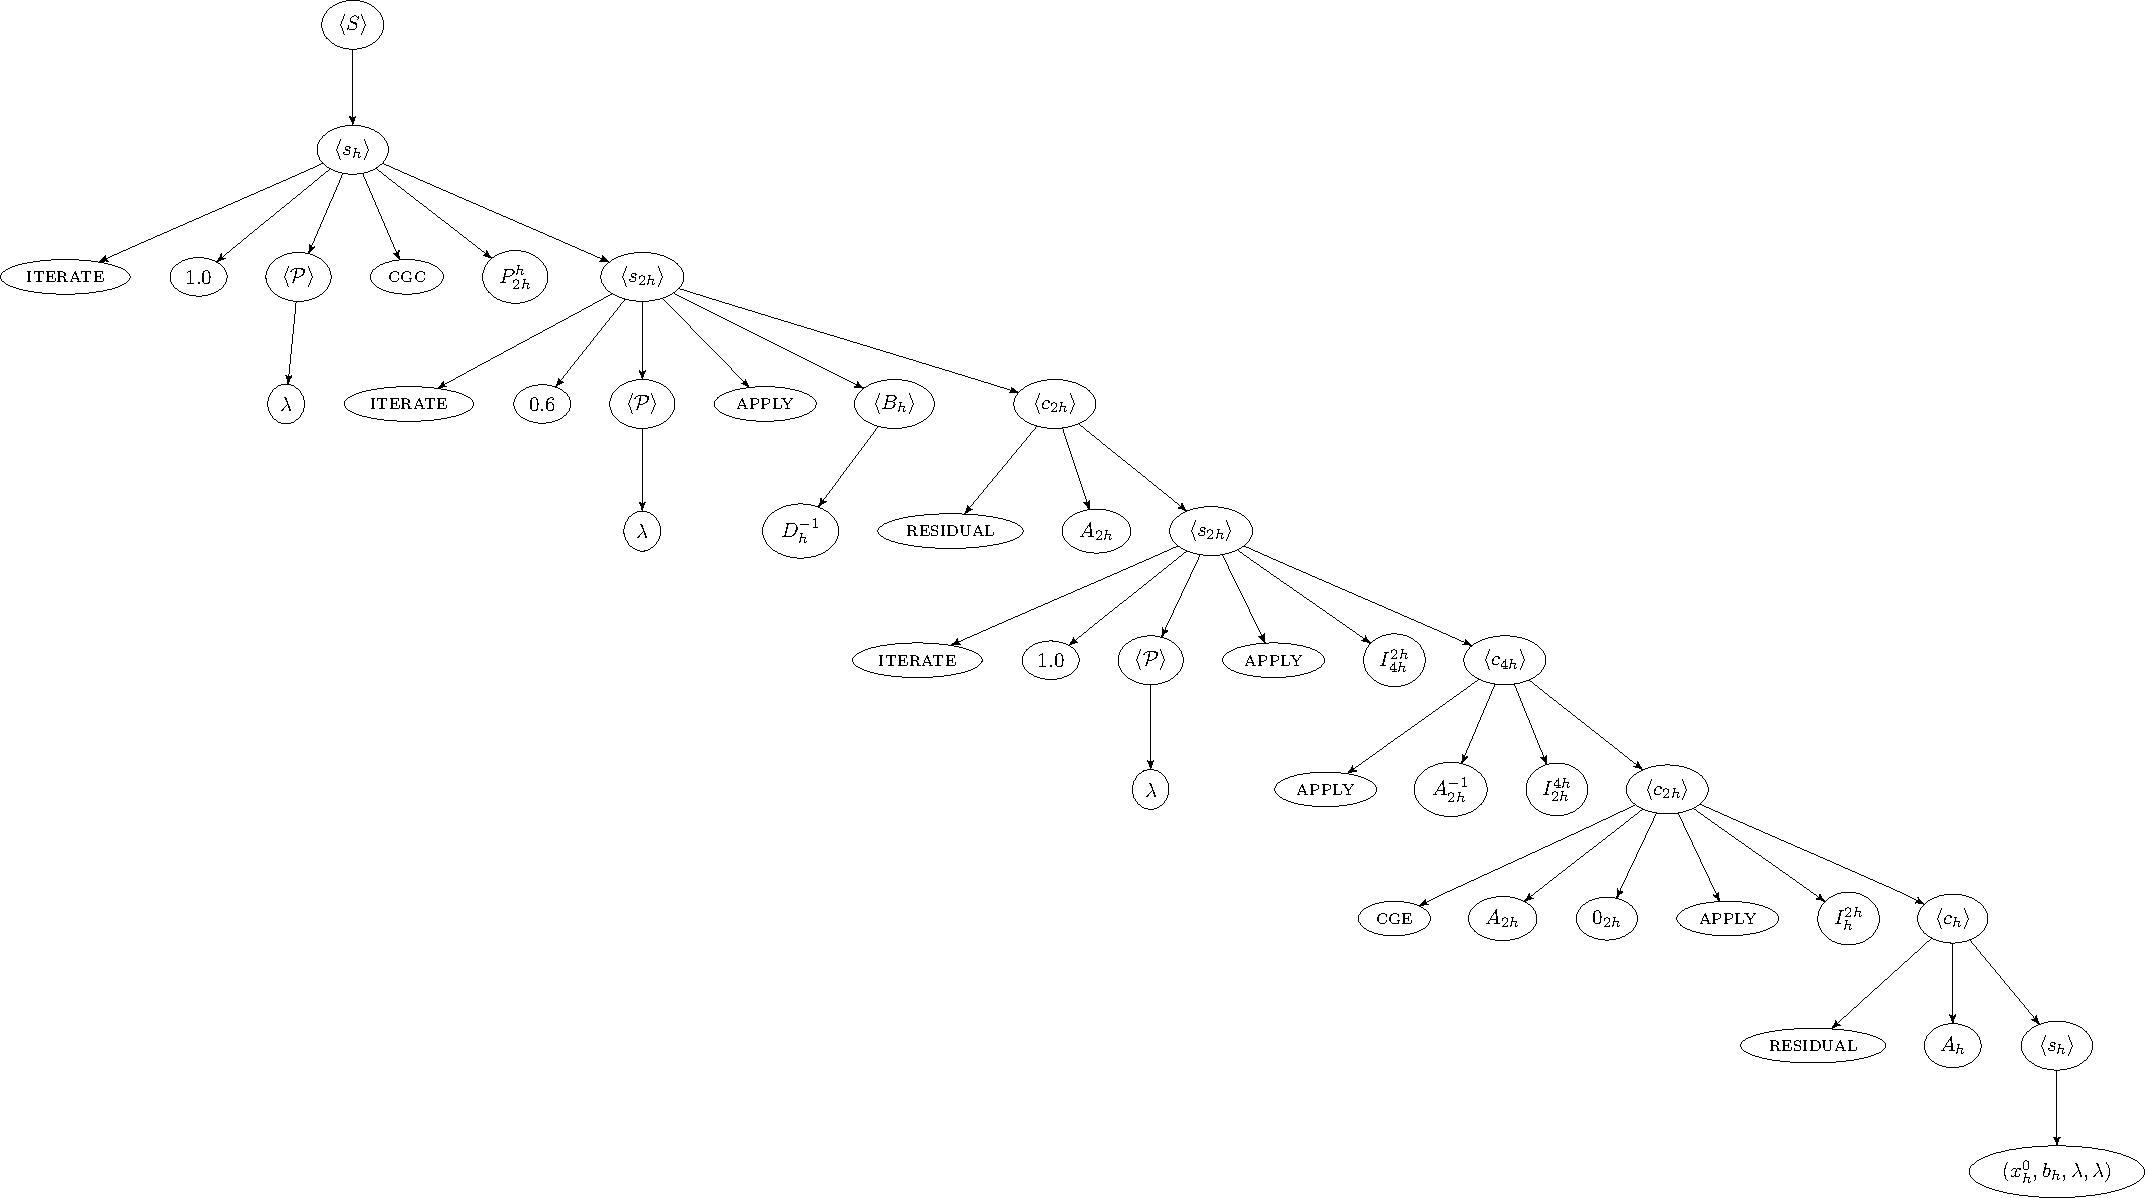
\includegraphics[width=\textwidth]{figures/trees/three_grid_method_grammar_tree.pdf}
	\caption{Grammar derivation tree for the three-grid method shown in Algorithm~\ref{alg:example-three-grid-method}.}
	\label{fig:example-three-grid-method-derivation-tree}
\end{figure}
Note that each inner tree node corresponds to a symbol contained in the set of variables $V$ of our grammar, as shown in Equation~\eqref{eq:multigrid-grammar-variables}, while all leaf nodes refer to terminals.
Since in the context of Table~\ref{table:multigrid-grammar}, the application order of each function is well-defined, we have omitted all parentheses in the tree for the sake of simplicity.
%TODO evtl darauf eingehen, dass der CGS auf dem entsprechenden level spezifiziert sein muss

Until now, we have been exclusively concerned with the problem of developing a formal representation for a multigrid method that is based on its algorithmic formulation.
However, in contrast to Figure~\ref{fig:example-three-grid-method-derivation-tree}, within an evolutionary program synthesis method, a derivation tree is usually generated by applying a sequence of productions in a randomly-chosen order, either to alter an already existing tree or to create a completely new one from scratch.
We, therefore, have to consider the task of deriving a method's algorithmic formulation exclusively based on its representation as a derivation tree using the semantic evaluation rules that apply to each of its nodes.
As we have seen in Section~\ref{sec:multigrid-state-transitions}, the application of each of the transition functions generated by our grammar returns a new state $Z_H$ consisting of a tuple $\left( \tilde{x}_{H}, b_{H}, c_{H}, Z_{H/2}\right)$, where $H$ is the discretization width on the current level.
Starting from the initial state tuple $\left(x_{h}^0, b_{h}, \lambda, \lambda\right)$ we can, therefore, apply the respective sequence of transition functions in a bottom-up manner until we arrive at the final state $\left(\tilde{x}_{h}, b_{h}, \lambda, \lambda\right)$.
As we have shown in Figure~\ref{fig:example-tree-grid-method-states} the first component $\tilde{x}_{h}$ of this tuple then combines all computational steps of the corresponding multigrid method in a single expression
\begin{equation}
	\begin{split}
		\tilde{x}_h = \; & x_{h}^0 + I_{2h}^h ((x_{2h}^0 + I_{4h}^{2h} A_{4h}^{-1} I_{2h}^{4h} (I_{h}^{2h}(b_{h} - A_h x_{h}^0) - A_{2h} x_{2h}^0)) \\
		& + 0.6 \cdot D_{2h}^{-1} (I_{h}^{2h}(b_{h} - A_h x_{h}^0) - A_{2h} \\
		& \cdot (x_{2h}^0 + I_{4h}^{2h} A_{4h}^{-1} I_{2h}^{4h} (I_{h}^{2h}(b_{h} - A_h x_{h}^0) - A_{2h} x_{2h}^0)))).
		\label{eq:example-three-grid-method-expression}
	\end{split}
\end{equation}
While this expression includes all information about the computational structure of the method, certain terms occur multiple times, which might lead the redundant computations.
We can, however, remove this redundancy by considering Equation~\eqref{eq:example-three-grid-method-expression} as a computational graph, where each node either corresponds to an arithmetic operation or to a predefined symbol, such as $x^0_h$, $b_h$ and $A_h$.
The resulting graph for Equation~\eqref{eq:example-three-grid-method-expression} is shown in Figure~\ref{fig:example-three-grid-method-computational-graph}.
\begin{figure}
	\captionsetup{justification=centering}
	\begin{subfigure}[b]{0.49\textwidth}\centering
		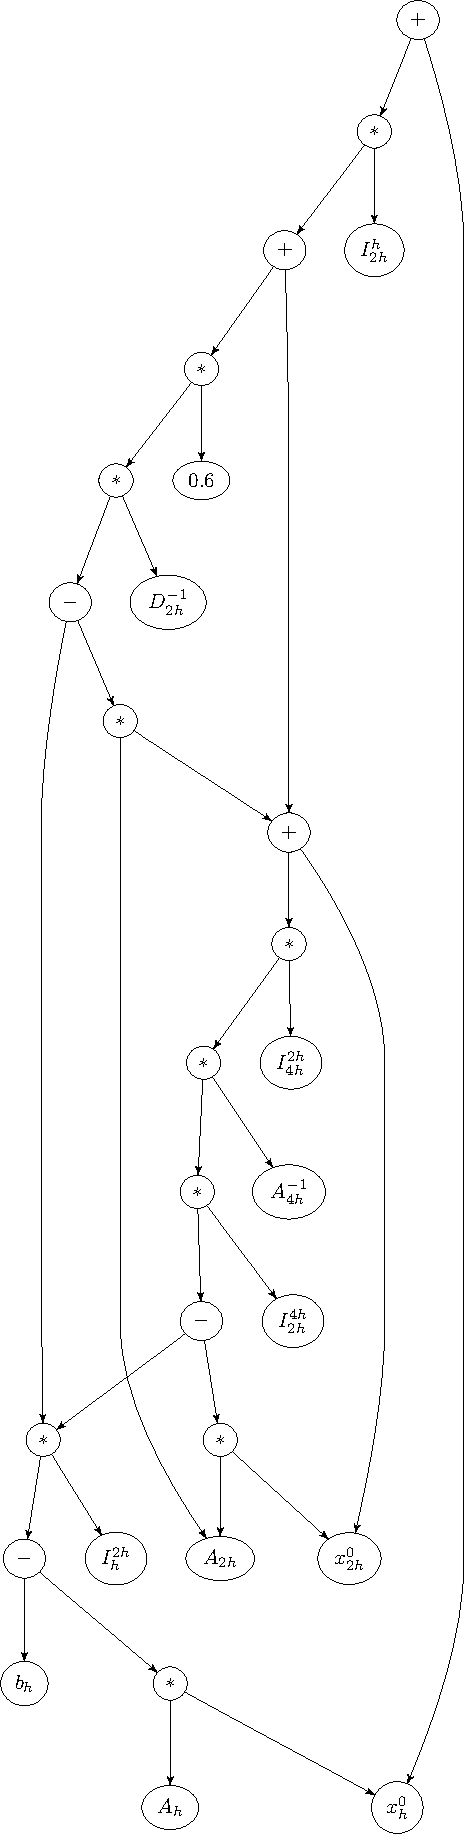
\includegraphics[scale=0.5]{figures/trees/three_grid_method_computational_graph.pdf}
		\caption{Original graph}
		\label{fig:example-three-grid-method-computational-graph-original}
	\end{subfigure}
	\begin{subfigure}[b]{0.49\textwidth}
 	\centering
		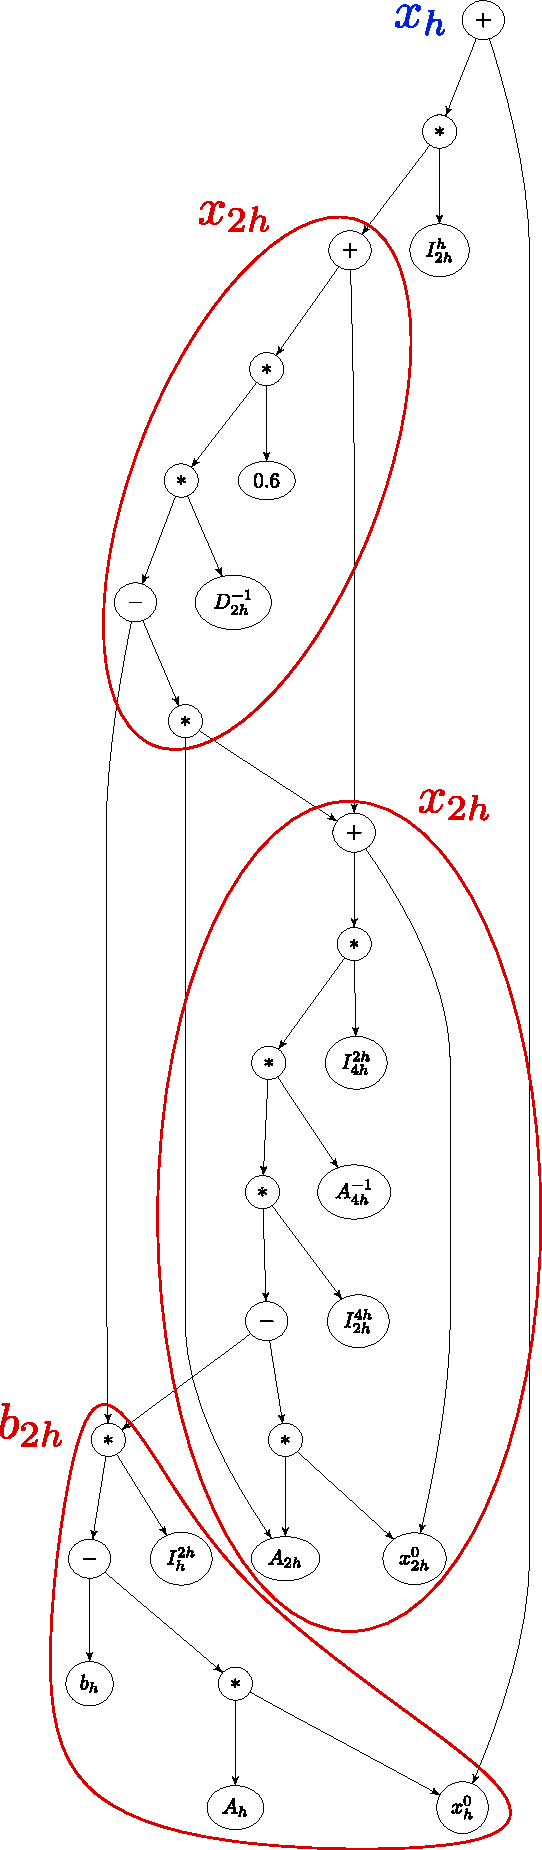
\includegraphics[scale=0.5]{figures/trees/three_grid_method_computational_graph_annotated.pdf}
		\caption{Annotated graph}
		\label{fig:example-three-grid-method-computational-graph-annotated}
	\end{subfigure}
	\caption{Computational graph for the three-grid method shown in Algorithm~\ref{alg:example-three-grid-method}.}
	\label{fig:example-three-grid-method-computational-graph}
\end{figure}
Again each node within this graph either corresponds to a predefined symbol or an operation defined on vectors and matrices, whereby in the case of the latter, there exists a direct edge to each node that refers to one of its arguments.  
Therefore, whenever a node serves as an argument to more than one operation, multiple edges are directed toward it.
Based on this representation, we can now define a redundancy-free sequence of computations that corresponds to the given multigrid method.
The most straightforward way to achieve this for a general graph is to simply introduce a temporary value for each non-leaf node of the graph.
However, note that every intermediate result in graph~\ref{fig:example-three-grid-method-computational-graph} that serves as an argument to multiple nodes refers to a term representing the computation of an approximate solution or right-hand side on the respective level.
To verify this assumption, consider again the three elementary multigrid operations listed in Definition~\ref{def:elementary-multigrid-operations}.
While a correction term is always discarded after its application, the current approximate solution is needed in the construction of the current residual as well as whenever its value is updated, either by means of smoothing or a coarse-grid correction.
Note that the same is true for the right-hand side, which is required whenever a new residual is constructed on a certain level.
This is illustrated in Figure~\ref{fig:example-three-grid-method-computational-graph-annotated}, where we have annotated all subgraphs that correspond to the computation of an approximate solution or right-hand side.
Based on this graph, we can now easily obtain an algorithmic representation for a multigrid solver while avoiding redundant computations entirely.
For this purpose, we first determine which node does not have any incoming edge.
Since this node computes the final approximate solution, we mark it as $\tilde{x}_h$ in Figure~\ref{fig:example-three-grid-method-computational-graph-annotated}.
The expression that needs to be assigned to this variable is then generated by recursively visiting its children.
Note that since the graph is traversed beginning with the last operation of the multigrid method, the algorithmic instructions are generated in reverse order. 
To avoid redundant computations, whenever a node is reached that either corresponds to an approximate solution or a right-hand side, we have to ensure that the respective subgraph is only generated once and assigned to a separate variable, which can then be referenced in all subsequent expressions.
Finally, the process of algorithm generation is carried out until only nodes without any outgoing edges can be reached.
For Figure~\ref{fig:example-three-grid-method-computational-graph-annotated}, we, thus, obtain the algorithmic representation shown in Algorithm~\ref{alg:example-three-grid-method-generated}.
Note that this formulation is mathematically equivalent to the three-grid method shown in Algorithm~\ref{alg:example-three-grid-method}, whereby the only difference is that certain intermediate expressions, such as the residual, are not assigned to a variable.
\begin{algorithm}
	\begin{algorithmic}[1]
		\State $ b_{2h} = I_{h}^{2h} \left(b_{h} - A_h x_{h}^0 \right)$
		\State $ \tilde{x}_{2h} = x^0_{2h} + I_{4h}^{2h} A_{4h}^{-1} I_{2h}^{4h} \left(b_{2h} - A_{2h} x^0_{2h}\right)$
		\State $ \tilde{x}_{2h} = \tilde{x}_{2h} + 0.6 \cdot D_{2h}^{-1} \left(b_{2h} - A_{2h} \tilde{x}_{2h}\right)$
		\State $\tilde{x}_{h} = \tilde{x}_{h}  + I_{2h}^h \tilde{x}_{2h}$
	\end{algorithmic}
	\caption{Three-grid multigrid method generated based on Figure~\ref{fig:example-three-grid-method-computational-graph-annotated}}
	\label{alg:example-three-grid-method-generated}
\end{algorithm}
Since we can apply the same approach to any computational graph derived from a derivation tree of our multigrid grammar, we arrive at the following three-step procedure of algorithm generation:
\begin{enumerate}
	\item Construct a multigrid method in the form of its grammar derivation tree.
	\item Transform the derivation tree to a graph-based intermediate representation.
	\item Generate expressions for each approximate solution and right-hand side through recursive graph traversal.
\end{enumerate}
With the formulation of this approach, we have now outlined all necessary steps from the grammar-based generation of a multigrid method to its translation into an algorithmic representation, based on which can then apply these methods within numerical solvers.
However, we have yet to discuss how the individual steps of our approach, as described in this section, can be carried out in an automatic way on a modern computer.
In the remaining part of this thesis, we will close this gap by presenting the implementation of our evolutionary program synthesis framework \emph{EvoStencils}, which is freely available as an open-source software library\footnote{EvoStencils: \url{https://github.com/jonas-schmitt/evostencils}}.
Since the EvoStencils framework builds substantially on the techniques presented in Section~\ref{sec:gggp}, it is, however, necessary to first determine whether these methods are suitable for the given task or whether a mere brute-force search might already be sufficient to identify the single best method among the set of possible ones for a given problem.
For this purpose, we have to estimate the size of the search space that is created by the grammar formulated in Table~\ref{table:multigrid-grammar}, i.e., the number of different individuals that can be generated based on its productions.

\subsection{Search Space Estimation}
\label{sec:search-space-estimation}
If we treat the grammar-based design of multigrid methods as a search problem, the size of the search space spanned by the underlying grammar corresponds to the number of different methods that can be constructed based on its productions.
For a small search space, it can be feasible to simply enumerate and evaluate all possible solutions. 
Such an approach has the advantage that the best solution can be determined in a deterministic manner while heuristic search methods, such as those presented in Section~\ref{sec:gggp}, are, in general, not guaranteed to find it.
For this purpose, we consider the following simplified model estimation, which acts as a lower bound of the size of the search space of a five-grid hierarchy, as defined by the grammar formulated in Table~\ref{table:multigrid-grammar}. 
As we have discussed in Section~\ref{sec:multigrid-methods}, multigrid methods need to combine smoothing and coarse-grid correction steps to effectively reduce both the high and low-frequency components of the error.
While often in practice, multiple smoothing steps are employed, the application of a coarse-grid correction without any smoothing is rarely used on any level~\cite{trottenberg2000multigrid}.
To simplify the search space estimation, we, therefore, introduce the additional constraint that, on any level, the total number of smoothing steps is always greater or equal to the number of coarse-grid corrections.
We, furthermore, enforce that coarsening and correction can only be performed after smoothing, with the exception of the topmost level, where we additionally allow coarsening to be applied as a first operation.
Since, on the finest grid, the original system is solved, finding an optimal sequence of operations is of utmost importance for the efficiency of a multigrid method, and we, hence, want to enforce fewer constraints on the order of the individual operations.
Therefore, using the symbols $S$, $R$, and $P$ for smoothing, coarsening, and coarse-grid correction\footnote{For the sake of simplicity, we use the starting letters of restriction and prolongation as abbreviations for coarsening and coarse-grid correction.}, respectively, in each step of the method, depending on the level, the following sequences of operations can be defined:
\begin{align*}
	S | RS | SR & \quad \text{for} \; l = l_{max} \\
	A^{-1} & \quad \text{for} \; l = l_{min} \\
	S | SR | SP & \quad \text{otherwise}.
\end{align*}
Consequently, with the exception of the coarsest level, where the only allowed operation is the application of the coarse-grid solver, there always exist three different orderings of the available operations.
However, each step includes the application of a smoother, which additionally needs to be chosen.
Assuming the number of available methods for this purpose is $n$, which includes different types of smoothers, partitionings, and relaxation factors, this results in a total number of $3 \cdot n$ options in each step of the method.
While none of these constraints is included in our original grammar shown in Table~\ref{table:multigrid-grammar}, these simplifications enable us to derive a closed-form expression which then acts as a lower bound for the actual size of the search space.
We can obtain such an expression in the form of a finite sum of polynomials by considering the total number of smoothing steps that are supposed to be performed within a multigrid method, whereby we know that for each step, we need to choose from $3 \cdot n$ options independent of the level on which the operations are performed.
As a consequence, if our method incorporates $k$ smoothing steps, the total number of options is 
\begin{equation}
	N_{n,k} = (3 n)^k
	\label{eq:simplified-number-of-options}
\end{equation}
We can illustrate this expression by considering the corresponding decision tree, which is shown in Figure~\ref{fig:decision-tree} for $n = 2$.
\begin{figure}
	\centering
	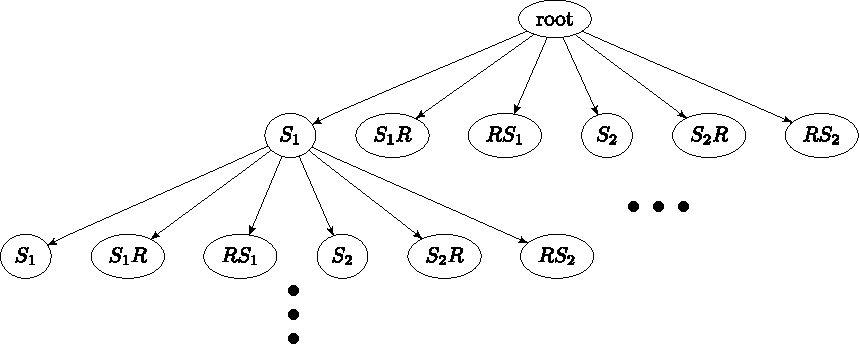
\includegraphics[width=\textwidth]{figures/trees/decision_tree_annotated.pdf}
	\caption{Simplified decision tree - Each node has the same number of children.}
	\label{fig:decision-tree}
\end{figure}
Each node in this tree corresponds to a particular choice of operations.
Since each step within our simplified decision model includes the application of either $S_1$ or $S_2$ as a smoother, which can then optionally be complemented with coarsening or coarse-grid correction, the depth of the tree is equal to the total number of smoothing steps $k$ applied within the multigrid method.
Each leaf of the tree, therefore, corresponds to a structurally-different multigrid method, and the total number of leaves is thus equal to $N_{2,k} = 6^k$.
However, since the optimal amount of smoothing is not known beforehand, we must consider a varying number of smoothing steps.
Now note that each decision tree that corresponds to a certain number of smoothing steps $k$ includes all those with fewer smoothing steps as a subtree, where each of these subtrees can be obtained by performing a top-down breadth-first traversal until the depth of the tree coincides with the respective number of smoothing steps.
Therefore, the total number of different multigrid methods with at least $k_{min}$ but at most $k_{max}$ smoothing steps is equal to the total number of leaf nodes of all subtrees of a decision tree of depth $k_{max}$ that have at least depth $k_{min}$.
Since the number of leaf nodes of a decision tree is given by Equation~\ref{eq:simplified-number-of-options}, the total number of different multigrid methods that employ between $k_{min}$ and $k_{max}$ smoothing steps is equal to
\begin{equation}
	N(n, k_{min}, k_{max}) = \sum_{k = k_{min}}^{k_{max}} N_{n,k} = \sum_{k = k_{min}}^{k_{max}} (3 n)^k.
	\label{eq:search-space-estimation}
\end{equation}
We can now finally make use of this formula to compute a lower bound for the total number of different five-grid methods that can be generated based on the grammar shown in Table~\ref{table:multigrid-grammar}.
For this purpose, we need to choose a reasonable interval for the minimum and maximum total number of smoothing steps of our method.
In Algorithm~\ref{alg:multigrid-cycle}, the total number of smoothing steps per level depends on the parameters $\nu_1$, $\nu_2$, and $\gamma$, which specify the number of pre-smoothing steps, post-smoothing steps and recursive descents per level, respectively.
Therefore, the total number of smoothing steps is given by
\begin{equation*}
	\sum_{k = 0}^{n_c - 1} \gamma^k (\nu_1 + \nu_2),
\end{equation*}
where $n_c$ is the number of coarsening steps.
%TODO only true for W-cycle, fix formula!
%TODO check if this has just been forgotten
Now let us consider how different choices of $\nu_1$, $\nu_2$, and $\gamma$ lead to a different total number of smoothing steps for a five-grid method ($n_c = 4$):
\begin{itemize}
	\item $V(1,0)$: $\gamma = 1, \nu_1 = 1, \nu_2 = 0 \Rightarrow 4 \; \text{smoothing steps}$
	\item $V(3,3)$: $\gamma = 1, \nu_1 = 3, \nu_2 = 3 \Rightarrow 24 \; \text{smoothing steps}$
	\item $W(1,0)$: $\gamma = 2, \nu_1 = 1, \nu_2 = 0 \Rightarrow 15 \; \text{smoothing steps}$
	\item $W(1,1)$: $\gamma = 2, \nu_1 = 1, \nu_2 = 0 \Rightarrow 30 \; \text{smoothing steps}$
	\item $W(3,3)$: $\gamma = 2, \nu_1 = 3, \nu_2 = 3 \Rightarrow 90 \; \text{smoothing steps}$
\end{itemize}
Setting $k_{min} = 4$ and $k_{max} = 30$ as an upper limit for the number of smoothing steps in Equation~\eqref{eq:search-space-estimation}, thus, represents a reasonable compromise since it allows us to generate multigrid methods that perform a similar amount of smoothing as the majority of commonly used $V$-cycles while methods comparable to less expensive $W$-cycle variants can also be obtained.
Finally, the only remaining parameter is the number of different methods available for each smoothing step.
To obtain a conservative estimate, we set $n = 2$, which means that in each step, we can only choose from two alternatives, for example, the Jacobi and red-black Gauss-Seidel method.
By utilizing Equation~\eqref{eq:search-space-estimation} we, thus, obtain 
\begin{equation*}
	N(2, 4, 30) = \sum_{k = 4}^{30} 6^k \approx 2.65 \cdot 10^{24}
\end{equation*}
as an estimated lower bound for the search space spanned by the grammar shown in Table~\ref{table:multigrid-grammar}.
If we now assume that a modern multi-core CPU is capable of evaluating each multigrid method on average in one millisecond,
even a supercomputer consisting of one trillion ($10^{12}$) such processors would require more than eight years to evaluate all methods contained in this search space.
Furthermore, in practice, it is usually beneficial to consider a higher number of different smoothers and relaxation factors, which results in an even larger search space.
As a consequence, while a pure brute-force-approach that aims to evaluate all possible multigrid methods may be feasible for the constrained parameter space that results from the classical formulation in Algorithm~\ref{alg:multigrid-cycle}, a grammar-based design requires the utilization of heuristic search method, such as those presented in Section~\ref{sec:gggp}.
\paragraph{Final Remarks}
In the remainder of this thesis, we will describe how G3P can be applied within \emph{EvoStencils}, our implementation of an automated grammar-based design method for multigrid methods in the Python programming language, which is based on the formal framework presented in this chapter.
We will, furthermore, demonstrate EvoStencils' effectiveness by evolving efficient multigrid methods for a number of different partial differential equations (PDEs).
In the following, we, therefore, assume a basic familiarity with Python due to its widespread use in both academia and industry.
If this should not be the case, the reader is advised to consult one of the many available resources for learning Python\footnote{Python:~\url{https://www.python.org/doc/}}.
We, furthermore, expect a basic knowledge of programming and parallelization techniques for recent multiprocessor and cluster systems, of which an overview can be found in~\cite{sterling2017high,hager2010introduction}.
%Furthermore, while hardware-specific code optimization is not a focus of this thesis, the reader should have some basic understanding about the architectural features of recent multiprocessor systems and supercomputers.
%Along with this, we also assume a familiarity with programming techniques and tools for performing a shared and distributed memory parallelization on these systems, such as OpenMP\footnote{OpenMP:~\url{https://www.openmp.org/}} and MPI\footnote{MPI:~\url{https://www.mpi-forum.org/}}. 
%\begin{figure}
%	\captionsetup{justification=centering}
%	\begin{subfigure}{0.1\textwidth}
%		\begin{tikzpicture}
%			\node   (h) at (-0.75, 4){$h$};
%			\node   (2h) at (-0.75, 3){$2h$};
%			\node   (4h) at (-0.75, 2){$4h$};
%			\node   (8h) at (-0.75, 1){$8h$};
%			\node   (16h) at (-0.75, 0){$8h$};
%		\end{tikzpicture}
%	\end{subfigure}
%	\begin{subfigure}{0.9\textwidth}
%		\begin{tikzpicture}
%			\node	(a) at (0,4) [draw, circle,fill=blue,scale=0.8] {};
%			\node	(b) at (0.5,3) [draw, circle, fill=blue, scale=0.8] {};
%			\node	(c) at (1,2) [draw, circle, fill=blue, scale=0.8] {};
%			\node	(d) at (1.5,1) [draw, circle, fill=blue, scale=0.8] {};
%			\node	(e) at (2,0) [draw, circle, ,fill=black, scale=0.8] {};
%			\node	(f) at (2.5,1) [draw, circle,scale=0.8] {};
%			\node	(g) at (3,2) [draw, circle,scale=0.8] {};
%			\node	(h) at (3.5,3) [draw, circle, scale=0.8] {};
%			\node	(i) at (4,4) [draw, circle,scale=0.8] {};
%			\draw 
%			(a) edge[->] (b) 
%			(b) edge[->] (c)
%			(c) edge[->] (d)
%			(d) edge[->] (e)   
%			(e) edge[->] (f)
%			(f) edge[->] (g)
%			(g) edge[->] (h)
%			(h) edge[->] (i)
%			;
%		\end{tikzpicture}
%	\end{subfigure}
%	
%	\caption{Five-grid cycle with $\nu_1 = 1$ and $\nu_2 = 0$. Smoothing is only performed in the steps corresponding to blue-colored nodes.}
%	\label{fig:five-grid-V-cycle}
%\end{figure}

